\chapter{Validierung}\label{sec:chapter7}

In diesem Kapitel werden die Ergbnisse des Vergleichs der ConDec - und BPMN-Modelle aus Kapitel 5 mit Hilfe einer Studie validiert.

\section{Forschungsfragen}

\textbf{Forschungsfrage 1a}: 

Ist die Punktsumme bei den Verständnisfragen insgesamt bei BPMN oder bei ConDec höher?\newline



\textbf{Forschungsfrage 1b}: 

Ist die Punktsumme bei den Verständnisfragen bei den kleinen Modellen bei BPMN oder bei ConDec höher?\newline

\textbf{Forschungsfrage 1c}: 

Ist die Punktsumme bei den Verständnisfragen bei den großen Modellen bei BPMN oder bei ConDec höher? \newline

\textbf{Forschungsfrage 1d}: 

Gibt es Unterschiede im Ergebnis in Abhängigkeit des Hintergrundwissesns der Versuchsobjekte über Prozessmodellierung?  \newline

\textbf{Forschungsfrage 2a}: 

Werden bei den Meinungsfragen insgesamt die Modelle von BPMN oder von ConDec präferiert? \newline

\textbf{Forschungsfrage 2b}: 

Werden bei den Meinungsfragen bei den kleinen Modellen die von BPMN oder von ConDec präferiert?\newline

\textbf{Forschungsfrage 2c}: 

Werden bei den Meinungsfragen bei den großen Modellen die von BPMN oder von ConDec präferiert?\newline

\section{Studie}

Abbildung \ref{fig:UmfrageStruktur} kann die Struktur der Umfrage entnommen werden.
Bei der Studie wurden zwei Fragebögen eingesetzt. Die 32 Teilnhemer der Studie wurden deswegen zufallsbedingt in zwei Gruppen (je 16 Personen) eingeteilt. Zunächst wurden den Probanden allgemeine demographische Fragen gestellt (Geschlecht, Alter, Hintergrundwissen zu imperativer und deklarativer Modellierung, Hintergrundwissen zu den Software Engineering Prozessmodellen Scrum, Open UP und V-Modell XT).\newline
Anschließend wurden den Teilnehmern Verständnisfragen zu ausgewählten Modellen gestellt.
Es wurden die vier  Modellpaare \textit{Lösungsinkrement entwickeln (Open UP)}, \textit{Scrum}, \textit{Systementwicklungsprojekt AG/AN} und \textit{Phasen Open UP -Inception}  aus Kapitel 5 ausgewählt. Hierbei wurde darauf geachtet, dass es sich um zwei kleine Modelle (<= 5 Aktivitäten) und zwei große Modelle (> 5 Aktivitäten) handelt. Gruppe 1 startete mit einem deklarativen Prozess und Gruppe 2 mit dem entsprechenden imperativen Prozess. Somit wurden von jeder Gruppe zwei imperative und zwei deklarative Prozesse bearbeitet.  \newline
Im letzten Teil des Fragebogens wurden den Probanden noch vier Modellpaare direkt gegenüber gestellt und sie wurden nach Ihrem präferierten Modell (deklarativ oder imperativ) gefragt und mussten in einem Freitextfeld den Grund für Ihre Entscheidung angeben. Auch hier wurden den Teilnehmern wiederum zwei kleine (<= 5 Aktivitäten) und zwei große (> 5 Aktivitäten)  Modelle gezeigt. Hier wurden die Modelle \textit{System spezifizieren (V-Modell XT)}, \textit{Phasen des Open UP}, \textit{Inkrementelle Entwicklung durchführen (V-Modell XT)} und \textit{Release deployen} ausgewählt. \newline
\begin{figure}[htp]
\begin{center}
  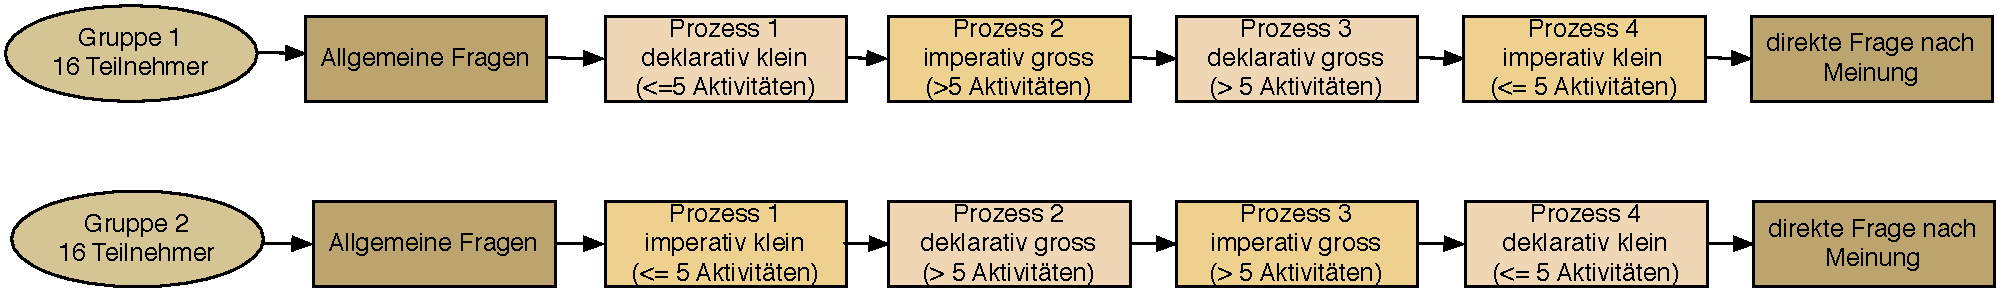
\includegraphics [width=\textwidth]{UmfrageStruktur} %pdf, jpg, png...
  \caption{Struktur der Umfrage}
  \label{fig:UmfrageStruktur}
\end{center}
\end{figure}

\subsubsection{Teilnehmer}

Es wurden 32 Studenten und Doktoranden aus dem Bereich Informatik/Medieninformatik befragt. 12 Teilnehmer waren weiblich und 20 männlich (Abbildung \ref{fig:Geschlechterverteilung}). Die allgemeinen demographischen Daten der Probanden können Abbildung \ref{fig:TabelleAllgemeineDaten} entnommen werden. Diese hatten unterschiedliches Hintergrundwissen zum Thema Prozessmodellierung. Wie Abbildung \ref{fig:VerteilungImperativDeklarative} entnommen werden kann, hatten sieben Studienteilnehmer weder in imperativer noch in deklarativer Modellierung Erfahrung. 18 Probanden hatten nur in imperativer Modellierung Erfahrung, jedoch nicht in deklarativer und sieben weitere Teilnehmer hatten in beiden Modellierungssprachen Erfahrung. Die Versuchsobjekte wurden bewusst nach unterschiedlichem Hintergrundwissen zum Thema Prozessmodellierung ausgewählt, um zu prüfen, inwiefern sich die Ergebnisse bei den Verständnisfragen zwischen Personen mit viel und wenig Hintergrundwissen zum Thema Prozessmodellierung unterscheiden.\newline

\subsubsection{Umfragewerkzeug und Durchführung}

Zur Durchführung wurde das Fragebogenwerkzeug \textit{Limesurvey} verwendet. Der entsprechende Link zum Fragebogen sowie eine kleine Legende zur Notationsübersicht von Declare und BPMN wurde den Teilnehmern per E-Mail zugeschickt. Die entsprechenden Antworten der Probanden wurden automatich von \textit{Limesurvey} gespeichert. Weiterhin war es dort möglich die jeweilige Zeit Zeit, welche die Probanden zur Bearbeitung Verständnisfragen benötigt haben, mit zu messen.

\begin{figure}[htp]
\begin{center}
  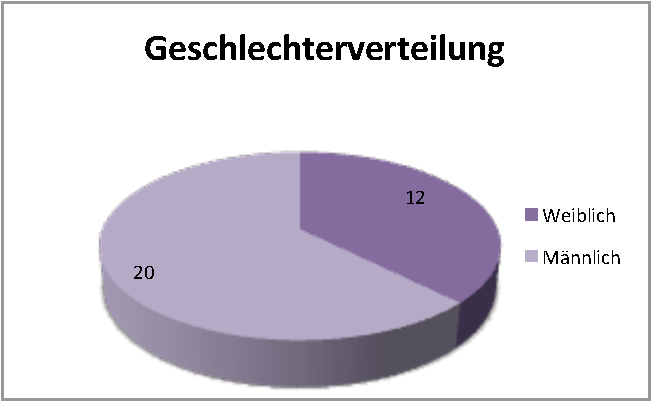
\includegraphics{Geschlechterverteilung} %pdf, jpg, png...
  \caption{Geschlechterverteilung}
  \label{fig:Geschlechterverteilung}
\end{center}
\end{figure}

\begin{figure}[htp]
\begin{center}
  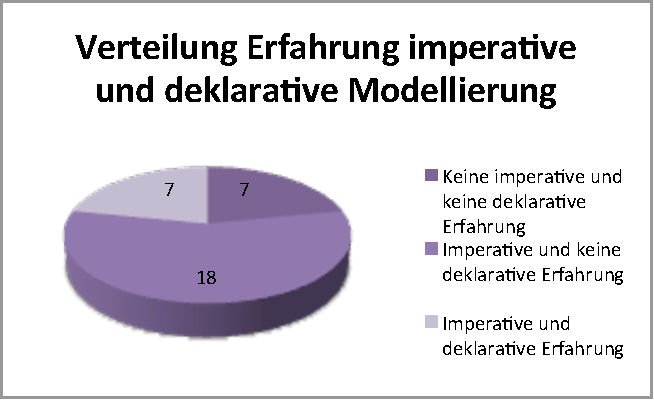
\includegraphics{VerteilungImperativDeklarative} %pdf, jpg, png...
  \caption{Verteilung Erfahrung imperative und deklarative Modellierung}
  \label{fig:VerteilungImperativDeklarative}
\end{center}
\end{figure}

\begin{figure}[htp]
\begin{center}
  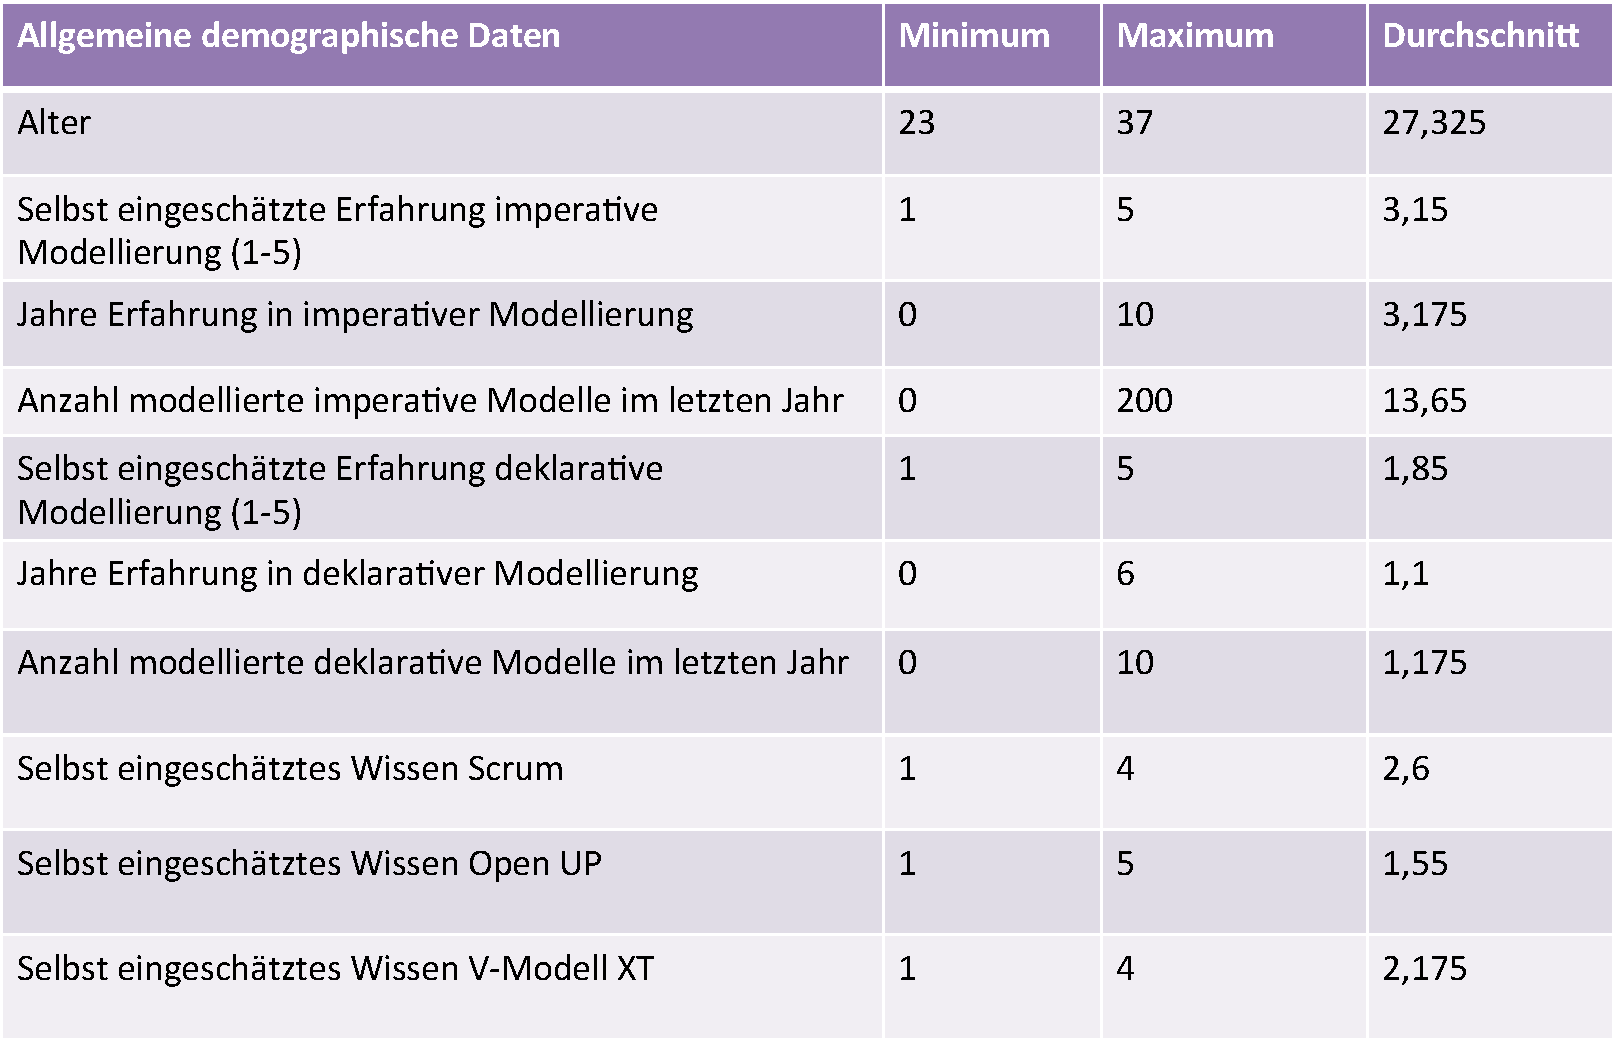
\includegraphics[width=\textwidth]{TabelleAllgemeineDaten} %pdf, jpg, png...
  \caption{Allgemeine demographische Daten}
  \label{fig:TabelleAllgemeineDaten}
\end{center}
\end{figure}









\subsubsection{Design der Studie}
Die Umfrage wurde online mit einem Fragebogen durchgeführt.
In einem ersten Teil